\documentclass[landscape,a0paper,fontscale=0.32]{baposter}

\usepackage{graphicx}
\usepackage{multicol}
\usepackage[utf8]{inputenc}
\usepackage{caption}

\newcommand{\compresslist}{%
\setlength{\itemsep}{1pt}%
\setlength{\parskip}{0pt}%
\setlength{\parsep}{0pt}%
}

\begin{document}
	\begin{poster}{background=none}
	{}
	{Row-Bot: Roboter essen Schmutz auf}
	{Simon Hüning}
	{
\includegraphics[width=0.2\linewidth]{pics/unilogo.png}}

		\headerbox{Hintergrund}{borderColor=yellow,headerColorOne=yellow,headerColorTwo=orange,name=problem,column=0,row=0}{
			Die Zeitdauer eines Roboters autonom, zu agieren ist limitiert. Z.B. muss der Energiebedarf ausreichend gedeckt sein, damit er funktioniert. Dies ist bei den meisten robotischen Systemen nur durch menschliche Handeln möglich. Für ein sich selbst mit Energie versorgendes System ergeben sich daraus folgende Vorraussetzungen:

			\begin{itemize}\compresslist
				\item Die Fähigkeit, selbstständig Energie zu produzieren
				\item Ein Betank- und Fortbewegungssystem, welches weniger Energie verbraucht, als produziert wird
			\end{itemize}
		}

		\headerbox{Die Ruderwanze}{borderColor=yellow,headerColorOne=yellow,headerColorTwo=orange,name=motivation,below=problem,column=0}{
				Eine ideales System generiert Energie aus der Umgebung, etwa wie Gewässer, in der es sich gerade befindet. Die Ruderwanze ernährt sich u.a. von den Algen aus den Gewässern, in denen sie lebt. Durch die Verdauung der Algen generiert sie Energie, durch die sich die Runderwanze weiter fortbewegen und neue Nahrung aufnehmen kann.				

				\hspace{1em}

				\begin{minipage}{1\linewidth}
					\centering
					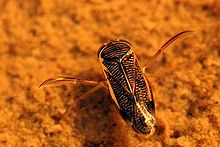
\includegraphics[width=1\linewidth]{pics/ruderwanze.png}
					\captionof{figure}{Ruderwanze}
				\end{minipage}

				\hspace{1em}

				\begin{minipage}{1\linewidth}
					\centering
					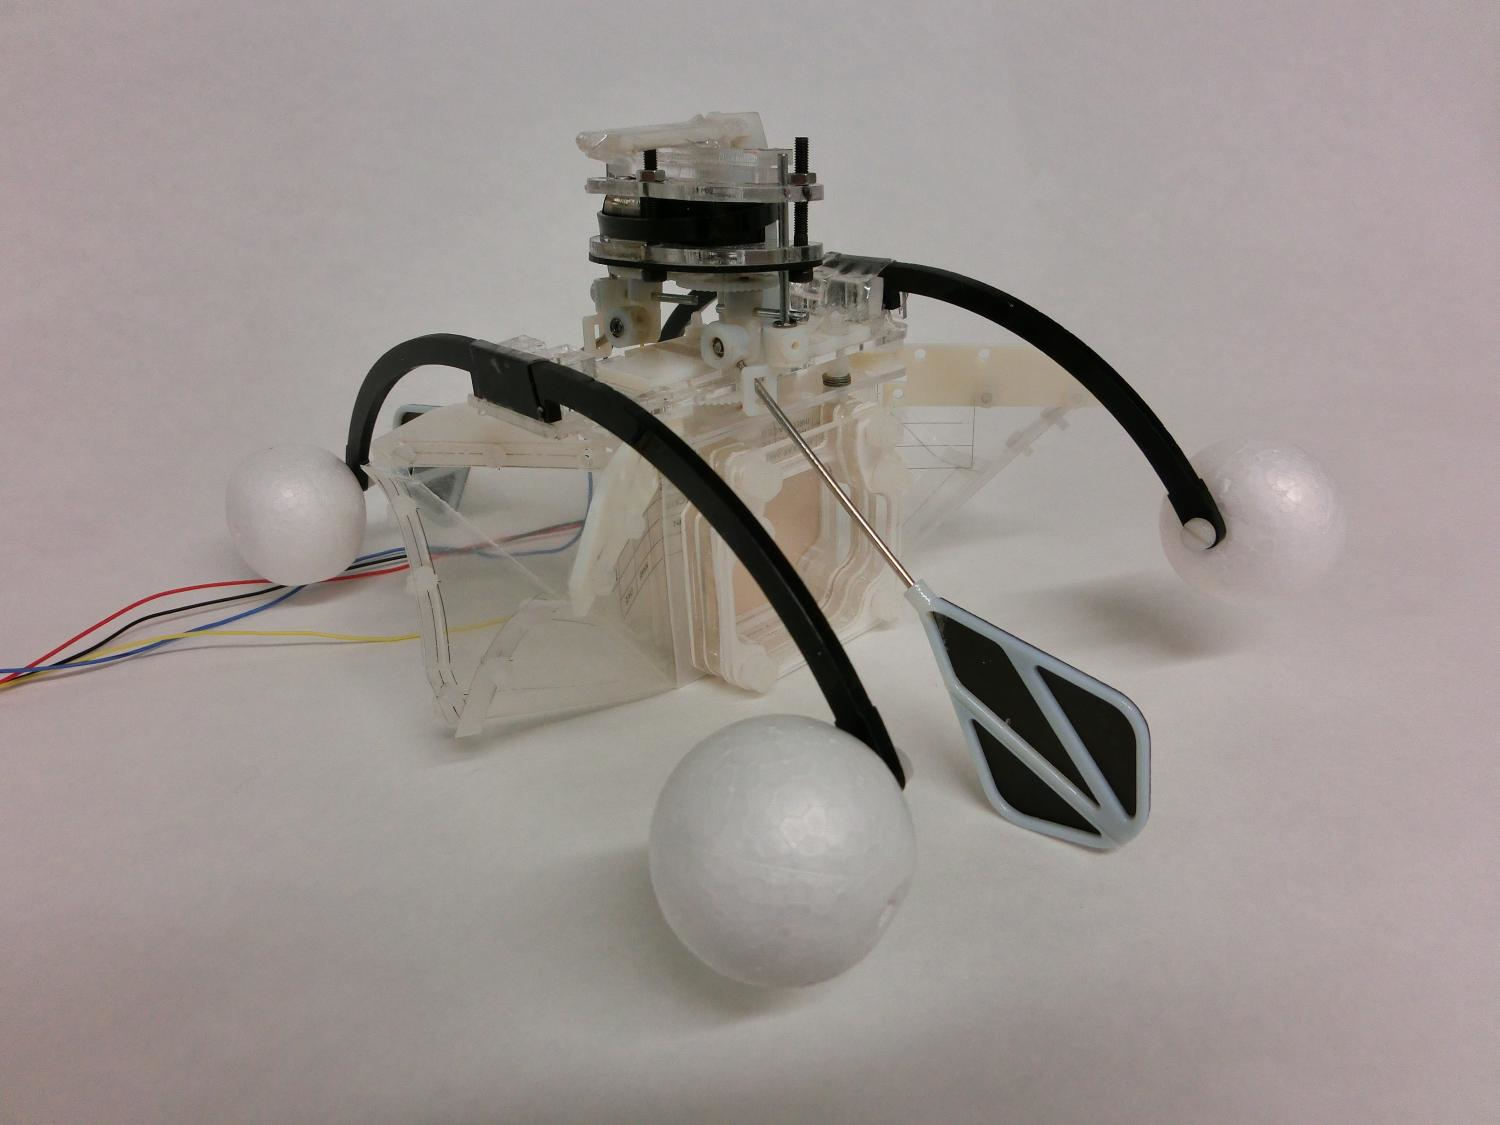
\includegraphics[width=1\linewidth]{pics/rowbot.png}
					\captionof{figure}{Row-Bot}
				\end{minipage}
		}

		\headerbox{Der Row-Bot}{borderColor=yellow,headerColorOne=yellow,headerColorTwo=orange,name=components,row=0,column=1,span=2}{
			\begin{multicols}{2}		
				\begin{minipage}{1\linewidth}
					\centering
					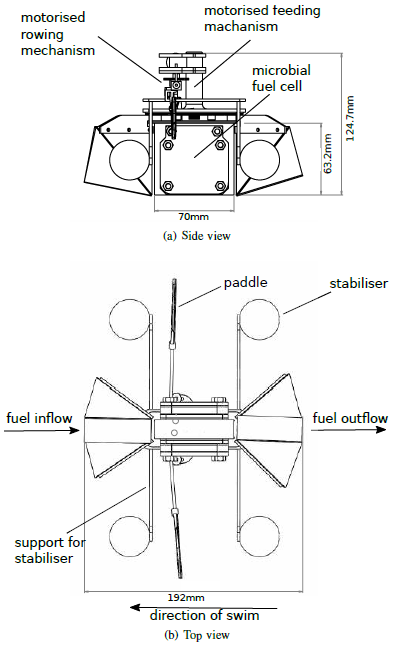
\includegraphics[width=.7\linewidth]{pics/schema.png}
					\captionof{figure}{Row-Bot-CAD-Modell}
				\end{minipage}
				
				\hspace{0.5em}

				Anterior und posterior an dem Row-Bot sind schließbare Öffnungen für den Zu- und Abfluss des Futters angebracht. Analog zur Runderwanze, welche schlagartige Bewegungen ihrer Hinterbeine nutzt, um sich im Wasser fortzubewegen, sind am Row-Bot seitlich Paddel angebracht. Nachdem sich der Mund geöffnet hat, beginnen die Paddel zu rudern, um neue Nährstoffe aus dem Wasser aufzunehmen. Nach einer gewissen Strecke bleibt der Bot stehen, schließt die Öffnungen wieder und beginnt mit der "Verdauung".

				\columnbreak
				
				\begin{minipage}{1\linewidth}
					\centering
					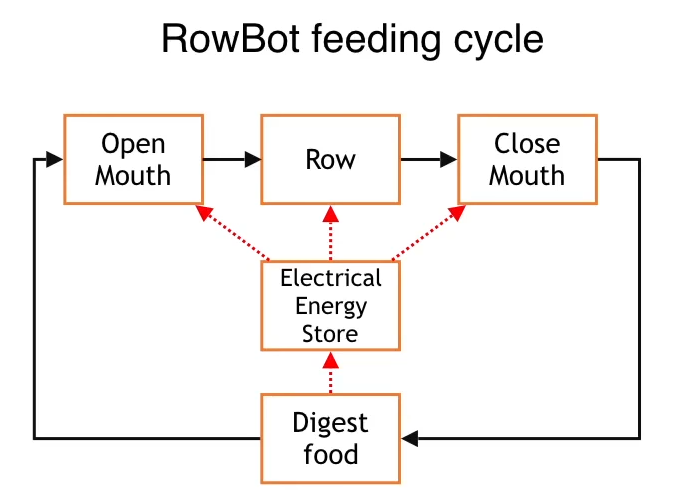
\includegraphics[width=0.9\linewidth]{pics/bewegungsablauf.PNG}
				\end{minipage}

				Eine mikrobielle Brennstoffzelle (MBZ) übernimmt die Funktion des Verdauungstraktes. Eine MBZ nutzt Mikroorganismen, die innerhalb ihres Stoffwechsels organische Substanzen verarbeiten. Durch den Stoffwechsel wird Strom erzeugt. Die Energie aus der MBZ wird genutzt, um zum einem den Ruder- und zum anderen den Fütterungsmechanismus zu betreiben.

				\hspace{0.5em}

				\begin{minipage}{1\linewidth}
					\centering
					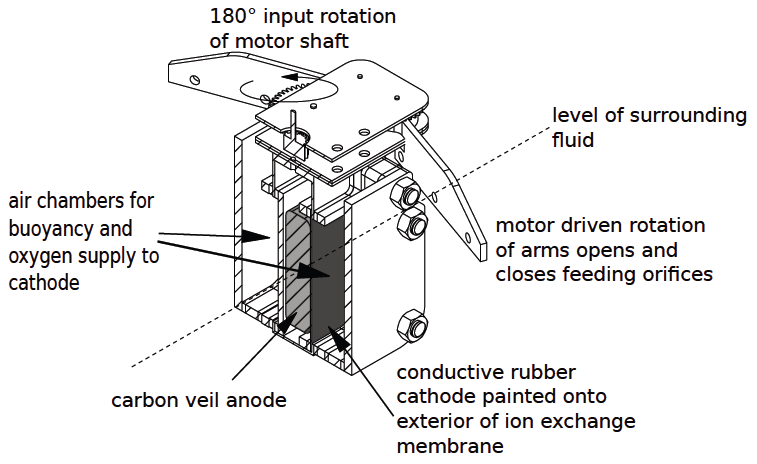
\includegraphics[width=1\linewidth]{pics/mfc.PNG}
					\captionof{figure}{Mikrobielle Brennstoffzelle}
				\end{minipage}
			\end{multicols}
		}

		\headerbox{Energiegewinnung}{borderColor=yellow,headerColorOne=yellow,headerColorTwo=orange,name=energy,below=components,column=1,span=2}{
			\begin{multicols}{2}

			Der Anodenraum der MBZ wurde mit 25ml Klärschlamm befüllt, welche man in 5 Folgetagen täglich mit 5ml Acetatlösung ersetzte. Danach zogen die Forscher die MBZ samt Füttersystem 20cm durch ein Wasserbecken, wo der Fütterzyklus vollzogen wurde.

			Ein Energiesammler wurde genutzt, um die geringe Spannung der MBZ auf 5,5V zu wandeln. Die MBZ würde über den Energiesammler eine Energie von 5J produzieren. Daraus lässt sich eine Kapazität eines Kondensators von 0,33F berechnen ($E=CV^2/2$). Die beobachtete Wandlungseffizienz des Konverters lag bei 30\%. Daraus resultierte eine reale Ladung von 4,1V. Bei dieser Wandlungseffizienz ist eine Kapazität von 0.18F nötig, um die gewünschten 5,5V zu erreichen.
			\columnbreak

			\begin{minipage}{1\linewidth}
				\centering
				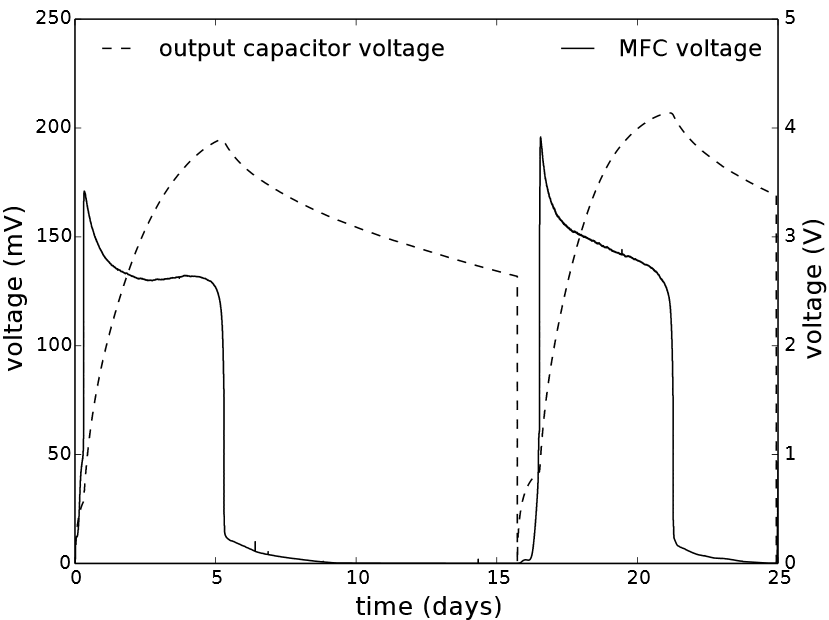
\includegraphics[width=0.9\linewidth,height=5cm]{pics/charge.png}
				\captionof{figure}{Voltoutput der MBZ und die entsprechende Voltladung des Energiesammlers}
			\end{minipage}

			\end{multicols}
		}

		\headerbox{Bewegung}{borderColor=yellow,headerColorOne=yellow,headerColorTwo=orange,name=movement,row=0,column=3}{
			Der Row-Bot wurde für den Bewegungstest in ein Wasserbecken gesetzt und jeweils einmal durch den mit 4,1V geladenen 0,33F und mit 5,5V geladenen 0,18F Kondensator betrieben. Die Bewegungen beinhalten den kompletten Futterzyklus. Nach Abschluss der Bewegungen blieben für den 0,33F Kondensator noch eine Restenergie von 0,58J und für den 0,18F Kondensator eine Restenergie von 0.9J.
			\begin{minipage}{1\linewidth}
				\centering
				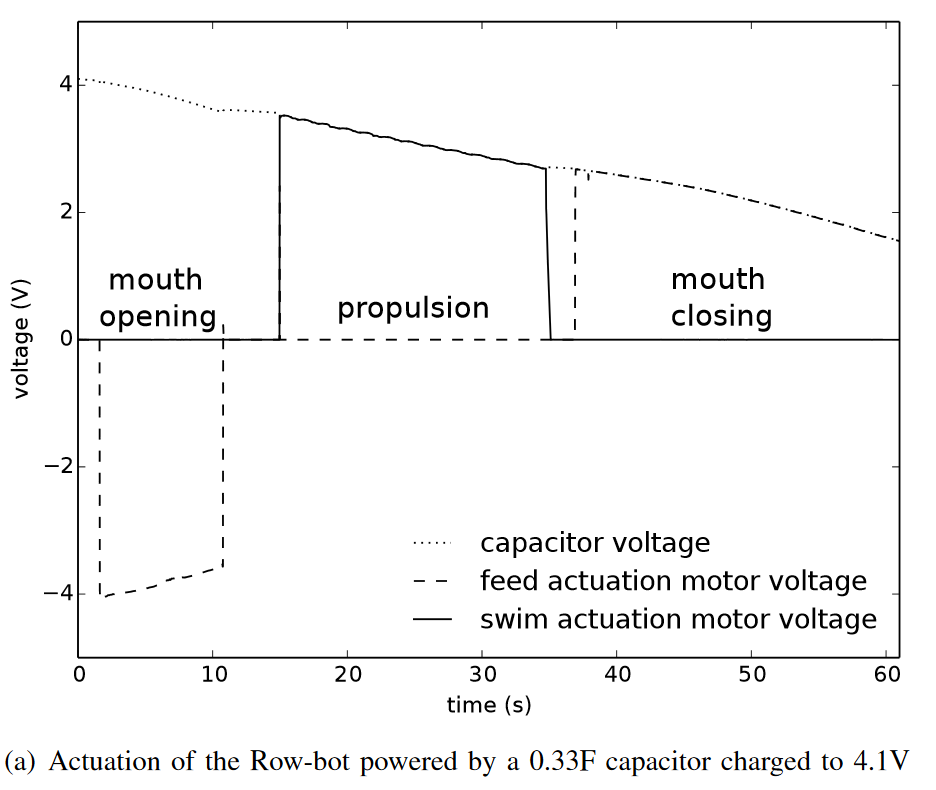
\includegraphics[width=0.8\linewidth,height=5.5cm]{pics/33.PNG}

				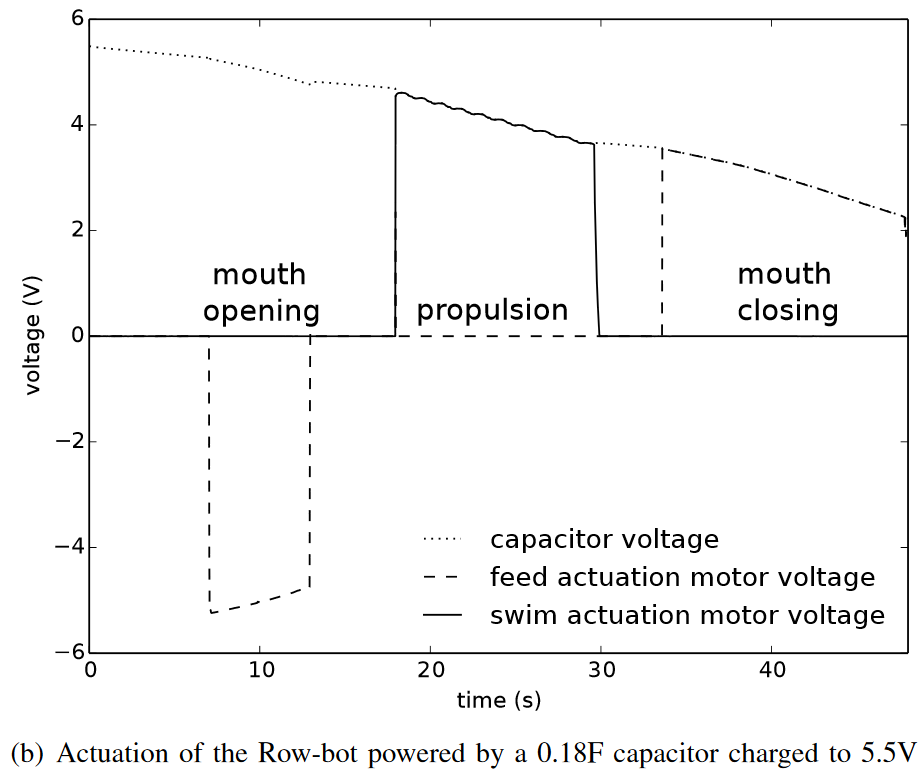
\includegraphics[width=0.8\linewidth,height=5.5cm]{pics/18.PNG}
				\captionof{figure}{Aktionen des Row-Bots}
			\end{minipage}
		}

		\headerbox{Schlussfolgerung}{borderColor=yellow,headerColorOne=yellow,headerColorTwo=orange,name=conclusion,below=components,above=bottom,column=3,span=1}{
			Der Resultate zeigen einen Roboter, der instande ist selbstständig Energie zu gewinnen und sich selbst wieder zu betanken. Die Bewegungseffizienz liegt noch weit hinter dem biologischem Vorbild, was sich mit einem Ruderschlag weiter fortbewegen kann. Dennoch zeigen die Messergebnisse eine Restenergie, die für weitere Aktionen genutzt werden kann, z.B. Positionsangabe. 

			Das langfristige Ziel der Entwickler ist der Einsatz des Row-Bots in verschmutzten Gebieten, wie riesige Algen- oder Ölteppiche in Meeren. Die Row-Bots sollen in Schwärmen durch ihre MBZ die Verschmutzungen eindämmen und säubern.
		}
	\end{poster}
\end{document}